\iffalse
\documentclass[journal,10pt,twocolumn]{article}
\usepackage{graphicx, float}
\usepackage[margin=0.5in]{geometry}
\usepackage{amsmath, bm}
\usepackage{array}
\usepackage{booktabs}
\usepackage[utf8]{inputenc}
\usepackage{amsfonts}
\usepackage{amssymb}
\usepackage{graphicx}
\usepackage{multicol}
\usepackage{tabularx}
\usepackage{hyperref}
\usepackage{mathtools}
\DeclareUnicodeCharacter{2212}{-}
\providecommand{\norm}[1]{\left\lVert#1\right\rVert}
\providecommand{\abs}[1]{\left\vert#1\right\vert}
\let\vec\mathbf
\newcommand{\myvec}[1]{\ensuremath{\begin{pmatrix}#1\end{pmatrix}}}
\newcommand{\mydet}[1]{\ensuremath{\begin{vmatrix}#1\end{vmatrix}}}
\providecommand{\brak}[1]{\ensuremath{\left(#1\right)}}
\providecommand{\lbrak}[1]{\ensuremath{\left(#1\right.}}
\providecommand{\rbrak}[1]{\ensuremath{\left.#1\right)}}
\providecommand{\sbrak}[1]{\ensuremath{{}\left[#1\right]}}
%\providecommand{\norm}[1]{\left\lVert#1\right\rVert}
%\providecommand{\sbrak}[1]{\ensuremath{{}\left[#1\right]}}
%\providecommand{\lsbrak}[1]{\ensuremath{{}\left[#1\right.}}
%\providecommand{\rsbrak}[1]{\ensuremath{{}\left.#1\right]}}
%\providecommand{\brak}[1]{\ensuremath{\left(#1\right)}}
%\providecommand{\lbrak}[1]{\ensuremath{\left(#1\right.}}
%\providecommand{\rbrak}[1]{\ensuremath{\left.#1\right)}}
%\providecommand{\cbrak}[1]{\ensuremath{\left\{#1\right\}}}
%\providecommand{\lcbrak}[1]{\ensuremath{\left\{#1\right.}}
%\providecommand{\rcbrak}[1]{\ensuremath{\left.#1\right\}}}
%\newcommand{\myvec}[1]{\ensuremath{\begin{pmatrix}#1\end{pmatrix}}}
%\let\vec\mathbf

\title{\textbf{Optimization-Basic Assignment}}
\author{Namrath Pinnamaneni \hspace{9cm} FWC22042}
\date{September 2022}

\begin{document}

\maketitle
\paragraph{\textit{Problem Statement} -
\fi
Find the maximum profit that a company can make if the profit function is given by  
\begin{align}
f(x) = 41-72x+18x^2
\end{align}
\\
\solution
\iffalse
A function f(x) is said to be convex if following inequality is true for $\lambda \in [0,1] :$  \label{opt/2/1/a/lemma1}
\begin{align}
    \lambda f(x_1) + (1-\lambda)f(x_2) \geq f(\lambda x_1 + (1-\lambda)x_2)
    \label{eq:12/6/5/62}
\end{align}
\fi
Considering
\begin{align}
    &\lambda\brak{41-72x_1-18x_1^2} + (1-\lambda)\brak{41-72x_2-18x_2^2} \geq \\
    &41-72\brak{\lambda x_1 + (1-\lambda)x_2} - 18\brak{\lambda x_1 + (1-\lambda)x_2}^2,
\end{align}
we obtain
\begin{align}
        18x_1^2\brak{{\lambda^2-\lambda}}+18x_2^2\brak{{\lambda^2-\lambda}}+36x_1x_2\brak{{\lambda^2-\lambda}} &\geq 0 \\
        x_1^2\brak{{\lambda^2-\lambda}}+x_2^2\brak{{\lambda^2-\lambda}}+2x_1x_2\brak{{\lambda^2-\lambda}} &\geq 0 \\
        -\lambda\brak{1-\lambda}\brak{x_1-x_2}^2 &\geq 0 \\
        \implies \lambda\brak{1-\lambda}\brak{x_1-x_2}^2 &\leq 0 \label{eq:12/6/5/67}
\end{align}
which is 
 false for all $\lambda\in(0,1)$. Hence the given function $f(x)$ is concave.
 \iffalse
 For a general quadratic equation
\begin{align}
    f(x)=ax^2+bx+c
\end{align}
\fi
    Using the gradient ascent method,
\begin{align}
    x_n=x_{n-1}+\mu\frac{df(x)}{dx} \label{eq:12/6/5/69}
    \end{align}
    Since
    \begin{align}
    \frac{df(x)}{dx}=-72-36x, \label{eq:12/6/5/610}
\end{align}
substituting \eqref{eq:12/6/5/610} in \eqref{eq:12/6/5/69}, 
\begin{align}
    x_n=x_{n-1}+\mu(-72-36x_{n-1})\label{eq:12/6/5/611}
\end{align}
Choosing
\begin{align}
	x_0 &= 1, \alpha = 0.001,  precision = 0.00000001, 
\\
	f_{max}  &\approx 113,
	x_{max}  \approx -2.0,
\end{align}
which is verified in Fig. 
		\ref{fig:12/6/5/6}.
	\begin{figure}[!ht]
		\centering
		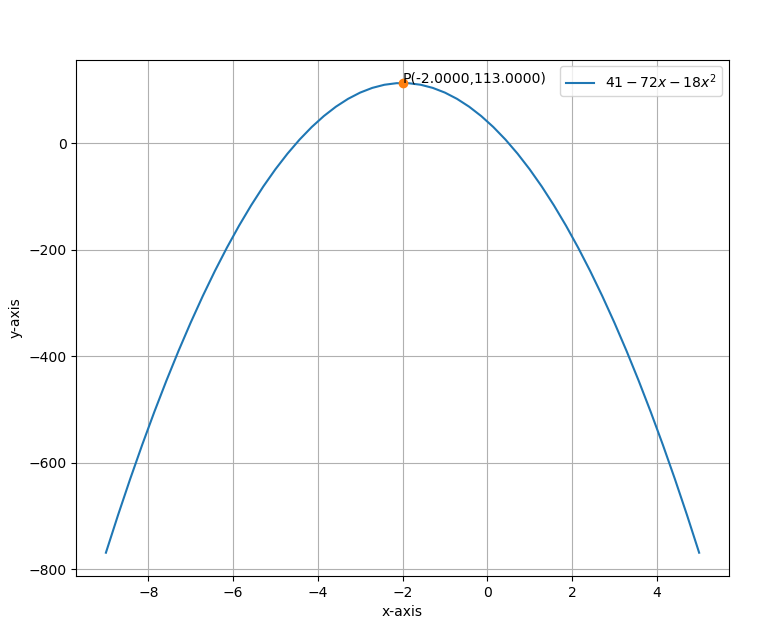
\includegraphics[width=\columnwidth]{12/6/5/6/figs/opt_basic.png}
		\caption{}
		\label{fig:12/6/5/6}
  	\end{figure}
\iffalse
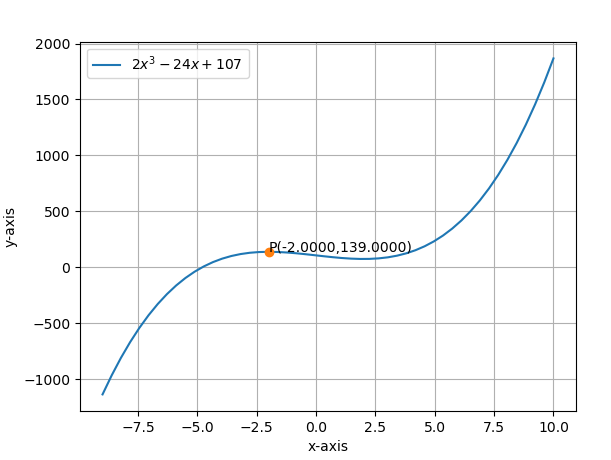
\includegraphics[width=1\columnwidth]{opt_basic.png}
\centering \text{Graph of f(x) = $41-72x+18x^2$}

\end{document}
\fi
